% Chapter 3

\chapter{DSL Specification with \textsc{Cinco}}\label{ch:DSL}

This chapter explains the specification underlying the user documentation model.  In our case, the specification is a textual DSL used to generate the graphical one. Section~\ref{sec:CTF} starts by giving a overview of the framework in use and the boilerplate code coming with it. It then continues with the main aspects of the \acrfull{mgl} and \acrfull{msl} as well as the \acrfull{cpd}. Finally, important key points of the Xtend generator classes are provided.

\section{\textsc{Cinco} SCCE Meta Tooling Framework}\label{sec:CTF}

The \textsc{Cinco} Framework is one of the many projects of the \href{https://www.scce.info/}{SCCE Group}, which aims at allowing the application experts, rather than programming experts, to take charge of the development tasks~\cite{scce}. It is a generator-driven development environment for graphical domain-specific modeling tools. As for many software frameworks, the purpose is to ease the development process by hiding the complexity of the underlying APIs and also by offering a selective integration of custom user-written code. This way, reusability and application specificity are guarantied. The framework is based on the Eclipse Modeling Framework (EMF) and Graphiti Graphical Tooling Infrastructure~\cite{Cinco}. The widely spread Eclipse's Integrated Development Environment (IDE) provides the necessary support and a certain familiarity with the editor, which makes it easy to use for software development.
\begin{figure}[h]
    \centering
    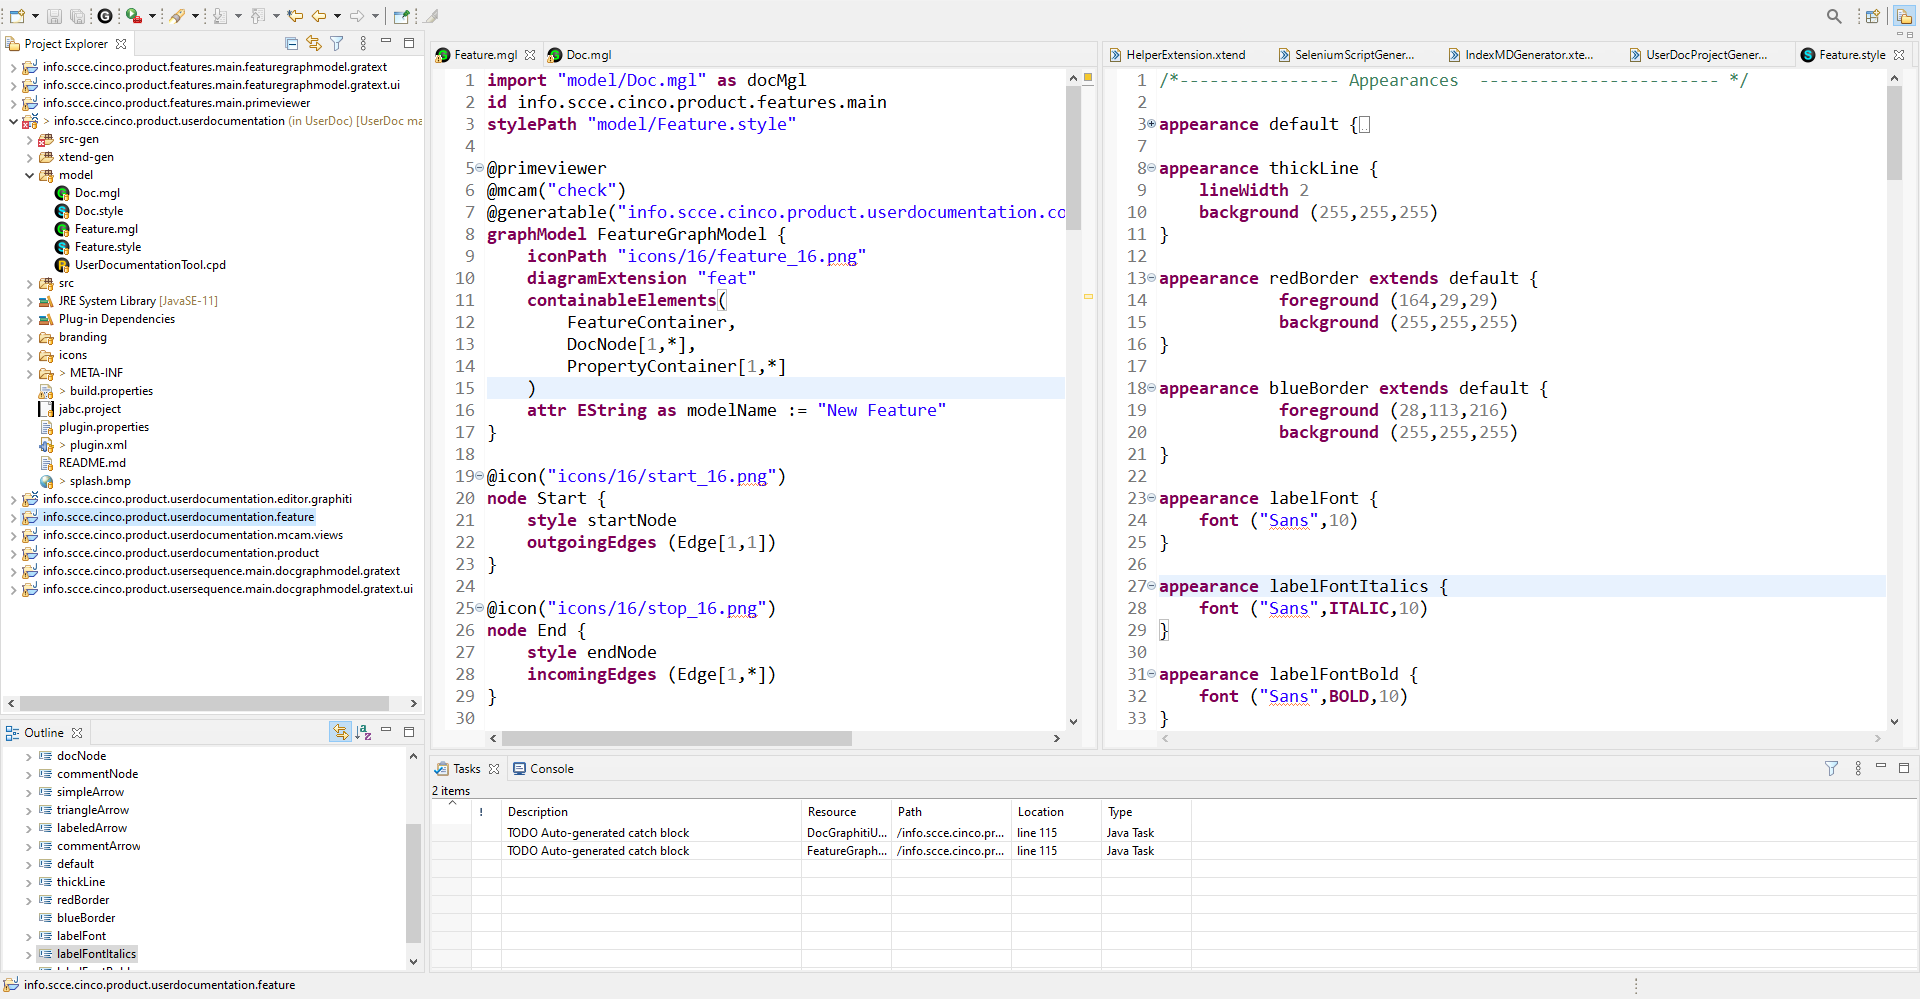
\includegraphics[width=\textwidth]{Cinco_EMF-Editor}
    \caption{The look of the Eclipse based \textsc{Cinco} IDE}
\end{figure}

The term \textit{Meta} indicates that the tooling suite proposes a solution for the elaboration of the meta-specification of the corresponding domain-specific modeling tool at metalevel. That means, the developer specifies the behavior and restrictions of the resulting graphical domain-specific modeling tool. Applying the concept of specialization at higher level brings much more control over the definition of the modeling tool and hence simplifies the development process. In this regard, the \textsc{Cinco} framework offers a push-button generation of the graphical tool editor~\cite{scce} right at meta-specification level. The generated editor instance is also an Eclipse-based editor, that can as well generate and execute programs on its turn, based on the tailored graphical model.

This automated generation of all the necessary application component creates a sets of plugins that carries extra functionalities to the editor application. For example, on creation of a new \textsc{Cinco} Product project, the developer has the possibility to include additional features she or he wishes to have for the development of the (meta)application. In our case for instance, we selected to have icons, appearance provider, code generation, product branding, custom actions and others. By doing so, the framework adds a set of packages containing classes with boilerplate code that can be extend with custom user-written code, as explained earlier. If we take the code generation feature for example, it adds the Generate Xtend class that implements the \textsc{Cinco} IGenerator (Xtend is a flexible and expressive dialect of Java, which compiles into readable Java 8 compatible source code~\cite{Xtend}). This class has to be passed as parameter of the annotation \lstinline[language=MGL]{@generatable("Generate.xtend")}. This class will be the entry point of the code generation process within the editor application.

As mentioned in the introduction, Xtext is used to define the textual syntax of the meta-specification that defines the appearance and structure of the model elements. This will not be discuss further as this will extrapolate the context of the thesis.  \textit{'Implementing Domain-Specific Languages with Xtext and Xtend'} by Lorenzo Bettini is a good reference for the interested reader to learn more about use of Xtext in DSL development. On the official \href{https://www.eclipse.org/Xtext/}{Eclipse website}, Xtext is defined as an open source framework for development of programming languages and domain-specific languages. Section \ref{sec:MGL}, \ref{sec:MSL} and \ref{sec:CPD} will offer an in-depth explanation on how this \acrshort{dsl} syntax is used to determine the look of each model element.

After writing down the textual specification comes the generation of the \textsc{Cinco} Product code. With each generation an Ecore object specific to each tool is also created to provide a description for the model and support needed at runtime. Ecore stands for \textit{\acrfull{emf} core}, which is the metamodel included in that framework. In addition, a corresponding editor based on Graphiti framework is created as well. It enables the creation, visualization and manipulation of the resulting model elements. Like most framework used in \textsc{Cinco}, Graphiti is also build around the \acrshort{emf} to allow the creation of diagram editors for targeted graphical domain models. More about Graphiti can be found \href{https://www.eclipse.org/graphiti/}{here}.

The full generation process of a graphical modeling tool (of a \textsc{Cinco} Product Application) comprises four essential (meta) levels~\cite{Naujokat2018}. The first level, associated with the role Eclipse Developer, is where the Ecore.ecore and GraphitiDiagram.ecore metamodel are developed. The second level is where \textsc{Cinco} Developers of the Chair 5 for Programming Systems used the metamodel from the first level to develope the MGL.ecore and Style.ecore (actually corresponding to the MSL described in Sec. \ref{sec:MSL}), which in turns will become metamodel of the third specification level, where the \textsc{Cinco} Product Developers operate and also where this thesis work comes in. This means the Eclipse Developers are now at the meta-metalevel, the \textsc{Cinco} Developers at metalevel of the specification elaborated in this work. For the remainder of the chapters we will be focusing on the third and fourth specification level. Latter is the level where the \textsc{Cinco} Product Users use the generated graphical editor to create the domain specific models. 

\section{Meta Graph Language}\label{sec:MGL}

The \acrfull{mgl} sketches the behavior, the constraints and gathers the all the graphical components that will constitute the model elements that come in use in every graph diagram created in the modeling tool. As a \textsc{Cinco} Product developer, this is most likely the first place to start: the main elements that can be define in a \acrshort{mgl} are \textbf{nodes}, \textbf{containers} and \textbf{edges}. 

As illustrated below in listing~\ref{docMGL}, we first begin by determining the graph id (line~\ref{line:id}), that will be use as the package name containing all classes generated base on the herein specified nodes. Optionally, we could also import an external graph; in that case the import statement should come in first position as it is the case in our listing example. The imported graph gets a variable name specified by the keyword \lstinline[language=MGL]{as} and can be therefor reference throughout the entire code (cf.\ line~\ref{line:extRef}). While this seems to be a simple import statement, the result is of a great impact, since it allows the \textsc{Cinco} product user to simple integrate a whole graph model inside another by drag and dropping the target model file into the diagram of the destination model. This is an intelligent implementation of reusability. Next, we specify the style to be used for the graphical representation of each model element; line~\ref{line:styl} at global level and in line~\ref{line:styStart} and~\ref{line:styEnd} i.e.\ at node level. Note that the style defined at node level have to exist in a dedicated style file prior to assigning them here, otherwise a compile error is raised until the missing style is added and saved.

\begin{lstlisting}[language=MGL, caption={Doc.mgl for the user sequence graph model}, label=docMGL, escapechar=|, name=DocMGL]
    import "model/Doc.mgl" as docMgl |\label{line:extRef}|
    id info.scce.cinco.product.features.main |\label{line:id}|
    stylePath "model/Feature.style" |\label{line:styl}|

    @primeviewer
    @mcam("check")
    @generatable("info.scce.cinco.product.userdocumentation.codegen.Generate", "/src-gen/") |\label{line:annotation}|
    graphModel FeatureGraphModel { |\label{line:modelStart}|
        iconPath "icons/16/feature_16.png"
        diagramExtension "feat"
        containableElements(FeatureContainer,DocNode[1,*])
        attr EString as modelName := "New Feature"
        attr EString as description := "New Description"
    }|\label{line:modelEnd}|

    @icon("icons/16/start_16.png")
    node Start extends docMgl::StartNode { |\label{line:nodes}|
        style startNode |\label{line:styStart}|
        outgoingEdges (Edge[1,1])
    }

    @icon("icons/16/stop_16.png")
    node End extends docMgl::EndNode {
        style endNode |\label{line:styEnd}|
        incomingEdges (Edge[1,*])
    }

    @icon("icons/16/container_16.png")
    @palette("Container") |\label{line:paletteAnnotation}|
    container FeatureContainer {
        style featureContainer("${title}") |\label{line:formatstring}|
        containableElements(
            Start[1,1],
            End[1,1],
            DocNode[1,*]
        )
        attr EString as title := "New Feature"
        attr EString as description := "This is an example of a short documentation that will appear in the markdown file later on."
    }
    
    @doubleClickAction("info.scce.cinco.product.userdocumentation.action.DocNodeOpenSubmodel")
    node DocNode{
        style docNode("${mgl.modelName}")
        prime docMgl::DocGraphModel as mgl
        attr EBoolean as createScreenshots := true
        incomingEdges (*[1,*])
        outgoingEdges (Edge[1,*])
    }

    enum Browsers {
        firefox chrome Edge safari ie opera
    }

    edge Edge { |\label{line:edge}|
        style simpleArrow
    }
\end{lstlisting}

Then from line~\ref{line:modelStart} to~\ref{line:modelEnd} we define some important attributes of the graph model line the icon and the file extension to be used for visual representation in the graphical modeling tool, as well as the model name and a list of element that can be contained with the modeling canvas. More will be explain in coming chapters.


Last, from line~\ref{line:nodes} to the end, we define graph model nodes by associating an existing style in the file specified by the \lstinline[language=MGL]{stylePath} keyword and restricting the type and number of edges that can be connect from and to them. In our case, the start node can only have an outgoing edge of the type \lstinline[language=MGL]{Transition} and opposed to that the end node can only be connected one incoming transition edge. This forces more or less the use of single ''pathed'' sequences without ramification. Those constraints are enforced using multiplicity statements like in \acrfull{uml} diagrams. In the same manner, container nodes can be given a style, attributes and incoming and/or outgoing edges with multiplicity constraints. In line~\ref{line:edge} we see a definition of the \lstinline[language=MGL]{edge} element that will connect model elements.

Additional elements like \lstinline[language=MGL]{enum} and user custom type introduced by keyword \lstinline[language=MGL]{type} can be added to create more tailored model elements. It is also possible to use annotation, which will be interpreted by external plugins, to add more functionality to node element. For example, line~\ref{line:annotation} shows a use of the \lstinline[language=MGL]{@generatable} annotation, which allows for code generation within the graphical editor. Here we give as parameter the Xtend class that will generate the code and the output folder.

For demonstration purposes, we kept our example listings short. An exhaustive list of all the usable elements and annotations can be found on the \textsc{Cinco}'s~\href{https://gitlab.com/scce/cinco/-/wikis/Cinco-Product-Specification}{Wiki page}, as well as a full description of the node elements created for our application in \ref{tab:listOfElements}.

\section{Meta Style Language}\label{sec:MSL}
The appearance of all the elements defined in the \acrshort{mgl} are laid down using the textual meta-language named \acrfull{msl}. As explained in~\cite{gitlabcinco}, three essential elements constitute the design of a \acrshort{msl} model, namely: \textbf{appearance}, \textbf{nodeStyle} and the \textbf{edgeStyle}.

Each nodeStyle specification makes use of an appearance element, which in fact determines the attributes like background color, the thickness of the drawn lines and so on. The beginning of listing~\ref{docStyle} shows the use of those attributes. It is also possible to control the appearance dynamically at runtime by associating to the concerned nodeStyle an appearance provider (cf.\ line~\ref{line:appearanceProvider}), which is in fact a Java or Xtend class implementing the \textsc{Cinco} meta core interface \lstinline{StyleAppearance}. The nodeStyle is hierarchically composed of a shape that can be given a \lstinline[language=MGL]{size}, \lstinline[language=MGL]{position} and a \lstinline[language=MGL]{text} element with a \lstinline[language=MGL]{value} attribute that takes a (format) string (line~\ref{line:shape}). Either the graph element in the \acrshort{mgl} using corresponding style has to provide a an attribute of type \lstinline{EString} that will be display in the graphical model (see line~\ref{line:formatstring} in listing~\ref{docMGL}) or the string provided by the value attribute is display. One other way to represent a node graphically is to use an \lstinline[language=MGL]{image} component instead of a shape element and provide a path to the image file -- like done for the \lstinline{screenshotNode} nodeStyle in line~\ref{line:image}.

\begin{lstlisting}[language=MGL, caption={Doc.style: styles to be applied to Doc.mgl}, label=docStyle, escapechar=|, name=docMSL]
    /*---------------- Appearances ------------------------*/

    appearance default { |\label{line:appearance}|
        lineWidth 1
        background (255,255,255)
    }

    appearance redBorder extends default { |\label{line:inheritance}|
        foreground (164,29,29)
        background (224,27,36)
    }

    appearance labelFont {
        font ("Sans",10)
    }

    /*---------------- Node Elements ------------------------*/

    nodeStyle startNode {
        roundedRectangle { |\label{line:shape}|
            appearance extends default {
                foreground (46,194,126)
                background (46,194,126)
            }
            position (0, 0)
            size (96, 32)
            corner (8, 8)
            text {
                position (CENTER, MIDDLE)
                value "Start"
            }
        }
    }

    nodeStyle endNode {
        roundedRectangle {
            appearance extends default {
                foreground (237,51,59)
                background (237,51,59)
            }
            position (0, 0)
            size (96, 32)
            corner (8, 8)
            text {
                position (CENTER, MIDDLE)
                value "End"
            }
        }
    }

    nodeStyle inputNode(1) {
        appearanceProvider("info.scce.cinco.product.userdocumentation.appearance.HighlightInputNodeAppearance") |\label{line:appearanceProvider}|
        roundedRectangle outer {
            appearance extends default {
                foreground (245,245,245)
                lineWidth 3
            }
            size(62,62)
            corner(8,8)
            roundedRectangle inner {
                appearance default
                position(CENTER,MIDDLE)
                size(60,60)
                corner(8,8)
                text {
                    position ( CENTER, MIDDLE )
                    value "%s"
                }
            }
        }
    }

    nodeStyle screenshotNode { |\label{line:image}|
        image {
            size (32, 32)
            path ("icons/32/browser_32.png")
        }
    }
\end{lstlisting}

Similarly, the edgeStyle is defined with an appearance component as well as a decorator. The appearance specifies the look of the edge line drawn in the diagram and the decorator draws the shape of the endings (see line~\ref{line:edgeStyle} in listing~\ref{docStyle2}). Possible shapes are ARROW, DIAMOND, CIRCLE and TRIANGLE\@.~\cite{gitlabcinco} offers a exhaustive documentation on the \textsc{Cinco} Product Specification.

It is also worth mentioning that the concept of inheritance from the \acrfull{oop} can be applied between metamodel element of the same type, hence avoiding repetitive definition of the same attributes within multiple different elements and allowing some elements to extends the properties of the parent elements. For example, we see in line~\ref{line:inheritance} the \lstinline{redBorder} appearance extends the default one and at the same time redefines the background color.

\begin{lstlisting}[language=MGL, caption={Doc.style part 2}, label=docStyle2, escapechar=|, name=docMSL]
    /*---------------- Edges ------------------------*/

    edgeStyle simpleArrow { |\label{line:edgeStyle}|
        appearance default

        decorator {
            location (1.0)
            ARROW
            appearance default
        }
    }

    edgeStyle commentArrow {
        appearance extends default {
            lineStyle DOT
        }

        decorator {
            location (1.0)
            ARROW
            appearance default
        }
    }
\end{lstlisting}

\section{Cinco Product Definition}\label{sec:CPD}

The \acrfull{cpd} offers an entry point when it comes to generating the application code. Herein, the \textsc{Cinco} Product Developer has to provide key information like the \textsc{Cinco} product name, at least one or more \acrshort{mgl} files to be included into the generation process. Optionally, one can setup a splash screen with branding images, add a descriptive text about the application and specify plugins and/or features~\cite{gitlabcinco}.
The listing below gives an insight into the \acrshort{cpd} specification language.

\begin{lstlisting}[language=MGL, caption={UserDocumentationTool.cpd}]
    CincoProduct UserDocumentationTool {
        mgl "model/Feature.mgl"
        mgl "model/Doc.mgl"
        
        splashScreen "branding/splash.bmp" {
            progressBar (37,268,190,10)
            progressMessage (37,280,190,18)
        }
    
        image16 "branding/Icon16_dark.png"
        image32 "branding/Icon32.png"
        image48 "branding/Icon48.png"
        image64 "branding/Icon64.png"
        image128 "branding/Icon128.png"
        linuxIcon "branding/Icon512.xpm"
	
        about {
            text "UserDoc is a DSL-driven generator of end user documentation for web application. It is a bachelor thesis project developed with the Cinco SCCE Meta Tooling Suite ( http://cinco.scce.info )."
        }

        plugins {
            info.scce.cinco.product.userdocumentation.edit,
            info.scce.cinco.product.userdocumentation.editor
        }
    }
\end{lstlisting}

To generate the \textsc{Cinco} product after completion of the mandatory information, right-click in the project explorer on the~.cpd file, then on ``Generate Cinco Product''. Subsequently, a set of gratext and graphiti plugins (see~\ref{sec:CTF}) are generated, providing enhancements for the target editor like the aforementioned generate button or the dual perspective on the model diagram (both source code and graphical diagram). 

In order to start the actual \textsc{Cinco} Product application right-click on the project containing the~.mgl,~.style and~.cpd files and select ``Run as'' then ``Eclipse Application''. A new Eclipse IDE will start and after selecting the workspace, you can then create a new project and begin with the creation of a model graph. More to it in Chapter~\ref{ch:CP}.

\section{Xtend Generators}\label{sec:GEN}

So far we merely accomplished the ground plan of our target application, which is laying out the graphical syntax of each model element. Now comes the most intricate task the \textsc{Cinco} Product Developer has to fulfill: implementing the model semantic. 

This section introduces the concept of code generation with Java and Xtend classes, not to be confused with the generation process of the editor application components. The semantic generation approach utilizes Java's and Xtend's text templating feature which is based on the generation pattern used in the \acrfull{jabc}~\cite{model-driver-dev_jABC,jabc-home}. In fact, many generator classes in our example project implement and extends interfaces from the generator runtime and template package of the jABC \textsc{Cinco} metaplugin. One of which is the IGenerator interface from the runtime package, that ought to be implemented, for its abstract method \lstinline{generate}, which has to be overridden, is the target of the generate button in the graphical editor (see listing~\ref{generateClass}). Another one is the ProjectTemplate abstract class from the template package. This class offers an abstract method \lstinline{projectDescription}, that allows to generate a whole project structure, specifying project natures, required dependencies plus creating package and folder structure.

For our documentation application we need to create two folder structures: one will be the Selenium-Java application with the specific maven project structure. We apply the rule of convention over configuration and generate the Java project as recommended on the~\href{https://www.apache.org/}{Maven Apache} website and add Selenium as a dependency. The other project structure we generate by following convention is for the VuePress project, which in fact is the end result we aim to obtain. The generation of both project structures are inclined by the Xtend class UserDocProjectGenerator in the \lstinline[language=MGL]{createProject} method (see line~\ref{line:createProject} in the listing below).

\begin{lstlisting}[language=MGL, caption={Generate.xtend clas implementing the IGenerator infterface}, label=generateClass, escapechar=|]
    package info.scce.cinco.product.userdocumentation.codegen

    import info.scce.cinco.product.features.main.feature.FeatureGraphModel
    import de.jabc.cinco.meta.plugin.generator.runtime.IGenerator
    import org.eclipse.core.runtime.IProgressMonitor
    import org.eclipse.core.runtime.IPath

    /**
    * @author Mukendi Mputu
    */
    class Generate implements IGenerator<FeatureGraphModel> {

        /*	*/
        override generate(FeatureGraphModel model, IPath srcGenPath, IProgressMonitor arg2) {
            new UserDocProjectGenerator(model).createProject |\label{line:createProject}|
        }
        
    }
\end{lstlisting}

A platoon of Xtend and Java template class are additionally implemented to create configuration files, application class files and also markdown files with the content model by the documentation designer in the graph model. In chapter~\ref{ch:intro} section~\ref{sec:objectives} we provided a link to the Github repository, where the complete application code can be found.

\section{Additional Features}

Besides the aforementioned Xtend generators there are some additional feature a \textsc{Cinco} product developer can utilize to gain more control over the application behavior and functionalities. Inside the source folder \lstinline{src} of the Cinco project, the developer can add divers packages besides the generator package to reinforce constraints and model validation or establish a certain number of actions to be executed, e.g when saving or creating a model diagram. For instance, we have mentioned previously that the appearance of the model elements can be determined or modified at runtime; so the responsible Xtend class reside for example in the \lstinline{appearance} package under the \lstinline{src} folder. It is also possible to implement post-creation actions to take effect immediately after model instantiation for example under the \lstinline{hook} package.  

In the next chapters, we deliver an extended explanation of the generator and feature classes, while introducing our application as an on going example, where listings with concrete implementation examples will be depicted.